% Sample tex file for usage of iidef.sty
% Homework template for Inference and Information
% UPDATE: October 12, 2017 by Xiangxiang
% UPDATE: 22/03/2018 by zhaofeng-shu33
\documentclass[a4paper]{article}
\usepackage[T1]{fontenc}
\usepackage{amsmath, amssymb, amsthm}
% amsmath: equation*, amssymb: mathbb, amsthm: proof
\usepackage{moreenum}
\usepackage{mathtools}
\usepackage{url}
\usepackage{graphicx}
\usepackage{subcaption}
\usepackage{booktabs} % toprule
\usepackage[mathcal]{eucal}
\usepackage{dsfont}

\usepackage{setspace}  
\setstretch{1.6}








\theoremstyle{definition}
\newtheorem{definition}{Definition}[section]
\newtheorem{example}[definition]{Example}
\newtheorem{exercise}[definition]{Exercise}
\newtheorem{remark}[definition]{Remark}
\newtheorem{observation}[definition]{Observation}
\newtheorem{assumption}[definition]{Assumption}
\newtheorem{convention}[definition]{Convention}
\newtheorem{priniple}[definition]{Principle}
\newtheorem{notation}[definition]{Notation}
\newtheorem*{axiom}{Axiom}
\newtheorem{coa}[definition]{Theorem}
\newtheorem{srem}[definition]{$\star$ Remark}
\newtheorem{seg}[definition]{$\star$ Example}
\newtheorem{sexe}[definition]{$\star$ Exercise}
\newtheorem{sdf}[definition]{$\star$ Definition}
\newtheorem{question}{Question}




\newtheorem{problem}{Problem}
%\renewcommand*{\theprob}{{\color{red}\arabic{section}.\arabic{prob}}}
\newtheorem{rprob}[problem]{\color{red} Problem}
%\renewcommand*{\thesprob}{{\color{red}\arabic{section}.\arabic{sprob}}}
% \newtheorem{ssprob}[prob]{$\star\star$ Problem}



\theoremstyle{plain}
\newtheorem{theorem}[definition]{Theorem}
\newtheorem{Conclusion}[definition]{Conclusion}
\newtheorem{thd}[definition]{Theorem-Definition}
\newtheorem{proposition}[definition]{Proposition}
\newtheorem{corollary}[definition]{Corollary}
\newtheorem{lemma}[definition]{Lemma}
\newtheorem{sthm}[definition]{$\star$ Theorem}
\newtheorem{slm}[definition]{$\star$ Lemma}
\newtheorem{claim}[definition]{Claim}
\newtheorem{spp}[definition]{$\star$ Proposition}
\newtheorem{scorollary}[definition]{$\star$ Corollary}


\newtheorem{condition}{Condition}
\newtheorem{Mthm}{Main Theorem}
\renewcommand{\thecondition}{\Alph{condition}} % "letter-numbered" theorems
\renewcommand{\theMthm}{\Alph{Mthm}} % "letter-numbered" theorems


%\substack   multiple lines under sum
%\underset{b}{a}   b is under a


% Remind: \overline{L_0}



\usepackage{calligra}
\DeclareMathOperator{\shom}{\mathscr{H}\text{\kern -3pt {\calligra\large om}}\,}
\DeclareMathOperator{\sext}{\mathscr{E}\text{\kern -3pt {\calligra\large xt}}\,}
\DeclareMathOperator{\Rel}{\mathscr{R}\text{\kern -3pt {\calligra\large el}~}\,}
\DeclareMathOperator{\sann}{\mathscr{A}\text{\kern -3pt {\calligra\large nn}}\,}
\DeclareMathOperator{\send}{\mathscr{E}\text{\kern -3pt {\calligra\large nd}}\,}
\DeclareMathOperator{\stor}{\mathscr{T}\text{\kern -3pt {\calligra\large or}}\,}
%write mathscr Hom (and so on) 

\usepackage{aurical}
\DeclareMathOperator{\VVir}{\text{\Fontlukas V}\text{\kern -0pt {\Fontlukas\large ir}}\,}

\newcommand{\vol}{\text{\Fontlukas V}}
\newcommand{\dvol}{d~\text{\Fontlukas V}}
% perfect Vol symbol

\usepackage{aurical}








\newcommand{\fk}{\mathfrak}
\newcommand{\mc}{\mathcal}
\newcommand{\wtd}{\widetilde}
\newcommand{\wht}{\widehat}
\newcommand{\wch}{\widecheck}
\newcommand{\ovl}{\overline}
\newcommand{\udl}{\underline}
\newcommand{\tr}{\mathrm{t}} %transpose
\newcommand{\Tr}{\mathrm{Tr}}
\newcommand{\End}{\mathrm{End}} %endomorphism
\newcommand{\idt}{\mathbf{1}}
\newcommand{\id}{\mathrm{id}}
\newcommand{\Hom}{\mathrm{Hom}}
\newcommand{\cond}[1]{\mathrm{cond}_{#1}}
\newcommand{\Conf}{\mathrm{Conf}}
\newcommand{\Res}{\mathrm{Res}}
\newcommand{\res}{\mathrm{res}}
\newcommand{\KZ}{\mathrm{KZ}}
\newcommand{\ev}{\mathrm{ev}}
\newcommand{\coev}{\mathrm{coev}}
\newcommand{\opp}{\mathrm{opp}}
\newcommand{\Rep}{\mathrm{Rep}}
\newcommand{\Dom}{\mathrm{Dom}}
\newcommand{\loc}{\mathrm{loc}}
\newcommand{\con}{\mathrm{c}}
\newcommand{\uni}{\mathrm{u}}
\newcommand{\ssp}{\mathrm{ss}}
\newcommand{\di}{\slashed d}
\newcommand{\Diffp}{\mathrm{Diff}^+}
\newcommand{\Diff}{\mathrm{Diff}}
\newcommand{\PSU}{\mathrm{PSU}(1,1)}
\newcommand{\Vir}{\mathrm{Vir}}
\newcommand{\Witt}{\mathscr W}
\newcommand{\Span}{\mathrm{Span}}
\newcommand{\pri}{\mathrm{p}}
\newcommand{\ER}{E^1(V)_{\mathbb R}}
\newcommand{\prth}[1]{( {#1})}
\newcommand{\bk}[1]{\langle {#1}\rangle}
\newcommand{\bigbk}[1]{\big\langle {#1}\big\rangle}
\newcommand{\Bigbk}[1]{\Big\langle {#1}\Big\rangle}
\newcommand{\biggbk}[1]{\bigg\langle {#1}\bigg\rangle}
\newcommand{\Biggbk}[1]{\Bigg\langle {#1}\Bigg\rangle}
\newcommand{\GA}{\mathscr G_{\mathcal A}}
\newcommand{\vs}{\varsigma}
\newcommand{\Vect}{\mathrm{Vec}}
\newcommand{\Vectc}{\mathrm{Vec}^{\mathbb C}}
\newcommand{\scr}{\mathscr}
\newcommand{\sjs}{\subset\joinrel\subset}
\newcommand{\Jtd}{\widetilde{\mathcal J}}
\newcommand{\gk}{\mathfrak g}
\newcommand{\hk}{\mathfrak h}
\newcommand{\xk}{\mathfrak x}
\newcommand{\yk}{\mathfrak y}
\newcommand{\zk}{\mathfrak z}
\newcommand{\pk}{\mathfrak p}
\newcommand{\hr}{\mathfrak h_{\mathbb R}}
\newcommand{\Ad}{\mathrm{Ad}}
\newcommand{\DHR}{\mathrm{DHR}_{I_0}}
\newcommand{\Repi}{\mathrm{Rep}_{\wtd I_0}}
\newcommand{\im}{\mathbf{i}}
\newcommand{\Co}{\complement}
%\newcommand{\Cu}{\mathcal C^{\mathrm u}}
\newcommand{\RepV}{\mathrm{Rep}^\uni(V)}
\newcommand{\RepA}{\mathrm{Rep}(\mathcal A)}
\newcommand{\RepN}{\mathrm{Rep}(\mathcal N)}
\newcommand{\RepfA}{\mathrm{Rep}^{\mathrm f}(\mathcal A)}
\newcommand{\RepAU}{\mathrm{Rep}^\uni(A_U)}
\newcommand{\RepU}{\mathrm{Rep}^\uni(U)}
\newcommand{\RepL}{\mathrm{Rep}^{\mathrm{L}}}
\newcommand{\HomL}{\mathrm{Hom}^{\mathrm{L}}}
\newcommand{\EndL}{\mathrm{End}^{\mathrm{L}}}
\newcommand{\Bim}{\mathrm{Bim}}
\newcommand{\BimA}{\mathrm{Bim}^\uni(A)}
%\newcommand{\shom}{\scr Hom}
\newcommand{\divi}{\mathrm{div}}
\newcommand{\sgm}{\varsigma}
\newcommand{\SX}{{S_{\fk X}}}
\newcommand{\DX}{D_{\fk X}}
\newcommand{\mbb}{\mathbb}
\newcommand{\mbf}{\mathbf}
\newcommand{\bsb}{\boldsymbol}
\newcommand{\blt}{\bullet}
\newcommand{\Vbb}{\mathbb V}
\newcommand{\Ubb}{\mathbb U}
\newcommand{\Xbb}{\mathbb X}
\newcommand{\Kbb}{\mathbb K}
\newcommand{\Abb}{\mathbb A}
\newcommand{\Wbb}{\mathbb W}
\newcommand{\Mbb}{\mathbb M}
\newcommand{\Gbb}{\mathbb G}
\newcommand{\Cbb}{\mathbb C}
\newcommand{\Nbb}{\mathbb N}
\newcommand{\Zbb}{\mathbb Z}
\newcommand{\Qbb}{\mathbb Q}
\newcommand{\Pbb}{\mathbb P}
\newcommand{\Rbb}{\mathbb R}
\newcommand{\Ebb}{\mathop\mathbb E}
\newcommand{\Dbb}{\mathbb D}
\newcommand{\Hbb}{\mathbb H}
\newcommand{\cbf}{\mathbf c}
\newcommand{\Rbf}{\mathbf R}
\newcommand{\wt}{\mathrm{wt}}
\newcommand{\Lie}{\mathrm{Lie}}
\newcommand{\btl}{\blacktriangleleft}
\newcommand{\btr}{\blacktriangleright}
\newcommand{\svir}{\mathcal V\!\mathit{ir}}
\newcommand{\Ker}{\mathrm{Ker}}
\newcommand{\Cok}{\mathrm{Coker}}
\newcommand{\Sbf}{\mathbf{S}}
\newcommand{\low}{\mathrm{low}}
\newcommand{\Sp}{\mathrm{Sp}}
\newcommand{\Rng}{\mathrm{Rng}}
\newcommand{\vN}{\mathrm{vN}}
\newcommand{\Ebf}{\mathbf E}
\newcommand{\Nbf}{\mathbf N}
\newcommand{\Stb}{\mathrm {Stb}}
\newcommand{\SXb}{{S_{\fk X_b}}}
\newcommand{\pr}{\mathrm {pr}}
\newcommand{\SXtd}{S_{\wtd{\fk X}}}
\newcommand{\univ}{\mathrm {univ}}
\newcommand{\vbf}{\mathbf v}
\newcommand{\ubf}{\mathbf u}
\newcommand{\wbf}{\mathbf w}
\newcommand{\CB}{\mathrm{CB}}
\newcommand{\Perm}{\mathrm{Perm}}
\newcommand{\Orb}{\mathrm{Orb}}
\newcommand{\Lss}{{L_{0,\mathrm{s}}}}
\newcommand{\Lni}{{L_{0,\mathrm{n}}}}
\newcommand{\UPSU}{\widetilde{\mathrm{PSU}}(1,1)}
\newcommand{\Sbb}{{\mathbb S}}
\newcommand{\Gc}{\mathscr G_c}
\newcommand{\Obj}{\mathrm{Obj}}
\newcommand{\bpr}{{}^\backprime}
\newcommand{\fin}{\mathrm{fin}}
\newcommand{\Ann}{\mathrm{Ann}}
\newcommand{\Real}{\mathrm{Re}}
\newcommand{\Imag}{\mathrm{Im}}
%\newcommand{\cl}{\mathrm{cl}}
\newcommand{\Ind}{\mathrm{Ind}}
\newcommand{\Supp}{\mathrm{Supp}}
\newcommand{\Specan}{\mathrm{Specan}}
\newcommand{\red}{\mathrm{red}}
\newcommand{\uph}{\upharpoonright}
\newcommand{\Mor}{\mathrm{Mor}}
\newcommand{\pre}{\mathrm{pre}}
\newcommand{\rank}{\mathrm{rank}}
\newcommand{\Jac}{\mathrm{Jac}}
\newcommand{\emb}{\mathrm{emb}}
\newcommand{\Sg}{\mathrm{Sg}}
\newcommand{\Nzd}{\mathrm{Nzd}}
\newcommand{\Owht}{\widehat{\scr O}}
\newcommand{\Ext}{\mathrm{Ext}}
\newcommand{\Tor}{\mathrm{Tor}}
\newcommand{\Com}{\mathrm{Com}}
\newcommand{\Mod}{\mathrm{Mod}}
\newcommand{\nk}{\mathfrak n}
\newcommand{\mk}{\mathfrak m}
\newcommand{\Ass}{\mathrm{Ass}}
\newcommand{\depth}{\mathrm{depth}}
\newcommand{\Coh}{\mathrm{Coh}}
\newcommand{\Gode}{\mathrm{Gode}}
\newcommand{\Fbb}{\mathbb F}
\newcommand{\sgn}{\mathrm{sgn}}
\newcommand{\Aut}{\mathrm{Aut}}
\newcommand{\Modf}{\mathrm{Mod}^{\mathrm f}}
\newcommand{\codim}{\mathrm{codim}}
\newcommand{\card}{\mathrm{card}}
\newcommand{\dps}{\displaystyle}
\newcommand{\Int}{\mathrm{Int}}
\newcommand{\Nbh}{\mathrm{Nbh}}
\newcommand{\Pnbh}{\mathrm{PNbh}}
\newcommand{\Cl}{\mathrm{Cl}}
\newcommand{\diam}{\mathrm{diam}}
\newcommand{\eps}{\varepsilon}
\newcommand{\Vol}{\mathrm{Vol}}
\newcommand{\LSC}{\mathrm{LSC}}
\newcommand{\USC}{\mathrm{USC}}
\newcommand{\Ess}{\mathrm{Rng}^{\mathrm{ess}}}
\newcommand{\Jbf}{\mathbf{J}}
\newcommand{\SL}{\mathrm{SL}}
\newcommand{\GL}{\mathrm{GL}}
\newcommand{\Lin}{\mathrm{Lin}}
\newcommand{\ALin}{\mathrm{ALin}}
\newcommand{\bwn}{\bigwedge\nolimits}
\newcommand{\nbf}{\mathbf n}
\newcommand{\dive}{\mathrm{div}}
\newcommand{\<}{\left<}
\renewcommand{\>}{\right>}



\usepackage{algorithm}
\usepackage{algorithmic}


\newcommand{\OPT}{\mathrm{OPT}}



\numberwithin{equation}{problem}
% count the eqation by section countation


\DeclareMathOperator{\sign}{sign}
\DeclareMathOperator{\dom}{dom}
\DeclareMathOperator{\ran}{ran}
\DeclareMathOperator{\ord}{ord}
\DeclareMathOperator{\img}{Im}
\DeclareMathOperator{\dd}{d\!}
\newcommand{\ie}{ \textit{ i.e. } }
\newcommand{\st}{ \textit{ s.t. }}




\usepackage[thehwcnt = 5]{iidef}
\usepackage{tikz} % Required for tikzpicture environment
\thecourseinstitute{Tsinghua University}
\thecoursename{Discrete Optimistic}
\theterm{Fall 2024}
\hwname{Homework}
\usepackage{geometry}
\geometry{left=1.5cm,right=1.5cm,top=2.5cm,bottom=2.5cm}

\begin{document}

\courseheader
\name{Lin Zejin}
\rule{\textwidth}{1pt}
\begin{itemize}
\item {\bf Collaborators: \/}
  I finish this homework by myself. 
%   If you finish your homework all by yourself, make a similar statement. If you get help from others in finishing your homework, state like this:
%   \begin{itemize}
%   \item 1.2 (b) was solved with the help from \underline{\hspace{3em}}.
%   \item Discussion with \underline{\hspace{3em}} helped me finishing 1.3.
%   \end{itemize}
\end{itemize}
\rule{\textwidth}{1pt}

\vspace{2em}


\sloppy
\pagenumbering{arabic}

\begin{problem}
    (a) Reduce from  the instance of MAX-E3SAT-6.

    \begin{center}
        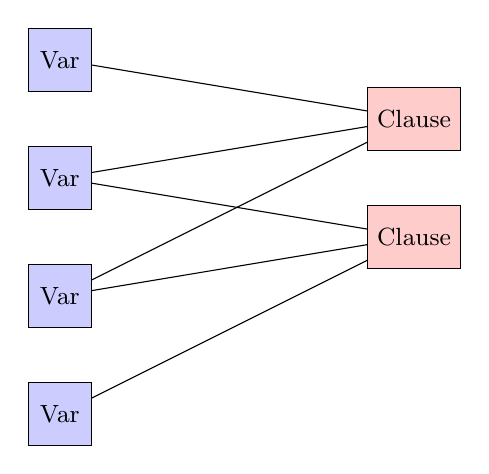
\begin{tikzpicture}[scale=1.5, every node/.style={draw, minimum size=0.8cm, font=\small}]
            % Variables (U)
            \node[fill=blue!20] (x1) at (0, 2) {Var};
            \node[fill=blue!20] (x2) at (0, 1) {Var};
            \node[fill=blue!20] (x3) at (0, 0) {Var};
            \node[fill=blue!20] (x4) at (0, -1) {Var};

            % Clauses (V)
            \node[fill=red!20] (c1) at (3, 1.5) {Clause};
            \node[fill=red!20] (c2) at (3, 0.5) {Clause};

            % Edges
            \draw[-] (x1) -- (c1);
            \draw[-] (x2) -- (c1);
            \draw[-] (x3) -- (c1);
            \draw[-] (x2) -- (c2);
            \draw[-] (x3) -- (c2);
            \draw[-] (x4) -- (c2);
        \end{tikzpicture}
        \end{center}
        Variables  $ x_i $ have  $ \sigma(x_i)\in \{0,1\} $ and Clauses  $ c_i=x_{j_i}^1\wedge x_{j_i}^2\wedge x_{j_i}^3 $ have  $ \sigma(c_i)\in [7] $ to represent the state of  $ c_i $. Therefore, constraint is naturally induced.

        In the instance of MAX-E3SAT, the radio of  $ |U| $ and  $ |V| $ is  $ 2 $. So this is a regular Label-Cover Game for  $ K=2,L=7 $ and  $ |V|=2|U| $.
         
        In the lecture we have proved that this is an instance of  $ \mathrm{MAX-LC}_{1,1-\epsilon} $ for some  $ \epsilon $.  

        So $ \mathrm{MAX-LC}_{1,1-\epsilon} $ is NP-Hard.


    (b)
    We actually can construct another graph induced by (a).

    We add  $ \bar{x}_i $ to the graph in  (a) and add the induced constraints from  $ c_i $ contains variable  $ x_i $ to  $ \bar{x}_i $.   
        
    Here the Label-Cover Game is regular and symmetric.

    Then for the  $ \mathrm{MAX-E3SAT-6}_{1,1-\epsilon} $ instance, the completeness is trivial.
    
    Now we prove the soundness. That's because, if  $ \OPT_{\mathrm{MAX-E3SAT-6}} \leq 1-\epsilon $, consider any  $ \sigma:U\rightarrow \{0,1\},V\rightarrow [7] $. At least  $ (1-\epsilon)|V| $ clauses are not satisfied by  $ \sigma|_U $. For each clause, there exists at least one variable  $ x_i/\bar{x}_i $ such that do not satisfy the constraint.
    
    So Verifier rejects with probability at least  $ (1-\epsilon)|V|/2|V|=(1-\epsilon)/2 $. So the soundness property holds if we set  $ \epsilon'=\frac{1+\epsilon}{2} $.
    
    So we prove that  $ \mathrm{GAP-LC}(K,L)_{1,1-\epsilon} $ is NP-Hard for some  $ \epsilon $  and  $ K,L $ even if the graph is regular and symmetric.
    
    By Raz' Paralled Repetition Theorem, we can reduce an instance of  $ \mathrm{GAP-LC}(K,L)_{1,\delta} $ to the instance of  $ \mathrm{GAP-LC}_{1,\exp(-\Omega(\frac{\delta^3t}{\log t}))} $. Therefore, we finally prove that for any  $ \eta>0 $, there exists  $ K,L $ such that  $ \mathrm{GAP-LP}(K,L)_{1,\eta} $ is NP-Hard.
        
\end{problem}

\begin{problem}
    (a) For a regular Label-Cover problem  $ G=(U,V,E) $ that every veritce in  $ U $ matches  $ k $ vertices in  $ V $,  $ |U|=|V|=n $ , consider the  $ k $-uniform hypergraph  $ H=(V',E') $ where  $ V'=E $ and  $ k $-tuples are all  $ [(u,v_1),(u,v_2),\cdots,(u,v_k)] $ for  $  (u,v_i)\in E   $.  $ [L'] $ now represents the value of $ (u,v_i) $, \ie    $ [L']=[L]\times [K] $.  $ [K]=[k+1] $. 
    
    The maps are defined as: For the labeling  $ \sigma:[V]\rightarrow[L]\times [K] $,  $ \sigma(u,v_i)=(l,k) $. If  $ \pi_{(u,v_i)}(k)=l $ is matching in Labek-Cover problem, then we let  $ \pi_e^i(\sigma(u,v_i))=k+1 $. Otherwise, if  $ (l,k) $ does not satisfy the constraint, then we let  $ \pi_e^i(\sigma(l,k))=i $.
    
    So the constraint is weakly satisfied iff at least two edges in the  $ k $-tuples are satisfied in the constraint before. Also, the constraint is strongly satisfied iff all edges in the  $ k $-tuples are satisfied.
    
    Completeness is trivial since if there is some label in the Label-Cover Game satisfy all constraint, then it can be naturally induced in the hypergraph.

    Soundness is because: Assume  $ \OPT \geq \epsilon $ in  $ k $-ary-Consistent-Labeling problem. Then we choose all edges  $ (u_i,v_j) $ that are satisfied in  the Label-Cover Game, denoted as  $ S $. There are at least  $ 2\epsilon n $ edges. Now we label each  $ u_i,v_j $ one by one.

    Since the graph  $ G $ is regular, at most  $ 2k-1 $   edges in  $ S $ have common vertice with an edge in  $ S $.
    
    So each time we choose an arbitrary  $ e=(u,v)\in S $, label it with the label in  $ k $-ary-Consistent-Labeling and then we remove those edges in  $ S $ who intersects with  $ e $.
    
    In the end, for those vertices that have not been labeled yet, label it randomly.

    Then at least  $ \frac{2\epsilon n}{2k}=\frac{\epsilon }{k}n $ edges are satisfied in Label-Cover-Game.
    
    Therefore  $ \OPT \geq \frac{\epsilon}{k} $ for Label-Cover Game.
    
    As a result, if  $ \OPT \leq \eta $ in Label-Cover Game, then  $ \OPT \leq k\eta $ in  $ k $-ary-Consistent-Labeling problem.
    
    Since  $ \mathrm{MAX-LC}_{1,\eta} $ is NP-Hard, to distingish instance with strong value $ 1 $ and weak value less than  $ k\eta $  $ k $-ary-Consistent-Labeling problem is NP-Hard  $ \forall \eta>0 $.
    
    Here we end the proof.

    (b)

    In  $ (a) $, we actually prove the $ l $-regular case: \ie each vertex  $ u $ appears in  $ l $  edges in the hypergraph.  

    For any hyperedge  $ e=(u_1,\cdots,u_k) $, let  $ T_e=\{1,2,\cdots,k\}^K $.
    
    The unverse is  $ W=\cup_{e\in E}T_e\times\{e\} $, and set 
    \[S_{u,\alpha}=\bigcup_{u\in e,e\in E}\{x\in T_e:x_{\pi_{i}(\alpha)}=i\text{ where }e_i=u\}\]
    Now we choose  $ |V| $ sets to cover this universe. 

    Completeness: If there is a instance with strong value  $ 1 $, of course the max-coverage is  $ 1 $.   

    Soundness: To prove if the instance has weak value less than  $ \delta $, then the max-coverage is less than  $ \epsilon+1-(1-\frac{1}{k})^k $. Suffices to prove that for each  $ \epsilon>0 $,  $ \exists \delta>0 $,   if the max-coverage value is larger than  $ \epsilon+1-(1-\frac{1}{k})^k $, then one can decode  $ \sigma $ such that  $ \mathrm{Val} \geq \delta $.

    \newcommand{\Sugg }{\mathrm{Sugg}}
    Let  $ \Sugg(u)=\{\alpha:S_{u,\alpha}\text{ is chosen}\} $.
    
    \begin{claim}
      \[\Ebb_{e\in E}\sum_{u\in e}|\mathrm{Sugg}(u)|=\frac{1}{|E|}\sum_{e\in E}\sum_{u\in e}|\mathrm{Sugg}(u)|=\frac{l}{|E|}\sum_{u}|\mathrm{Sugg}(u)|=k\]
      Here we use the  $ l $-regularity of the hypergraph, and  $ l|V|=k|E| $. 
    \end{claim}

    Denote 
    \[E_0=\{e\in E:\exists u,v\in e,u\neq v,\pi_{i(u)}(\Sugg(u))\cap \pi_{i(v)}(\Sugg(v))\neq \emptyset,\text{ where  $ i(u),i(v) $ is the position of  $ u,v $ in  $ e $}\}\]

    \[\tau=\Ebb_{e\in E_0}\sum_{u\in e}|\mathrm{Sugg}(u)|,\gamma=\frac{|E_0|}{|E|}\]

    For each  $ u $, if  $ \Sugg (u)\neq \emptyset $, then uniformly choose  $ \sigma(u)\sim \Sugg(u)  $, else if  $ \Sugg(u)=\emptyset $, choose  $ \sigma(u) $ arbitary.     
    \begin{claim}\label{claim}
      At least  $ \frac{k-1}{k} $ of edges in  $ |E_0| $ has the property that 
      \[\mathrm{Pr}[\text{weakly satisfied}] \geq \frac{1}{k^2\tau^2}\]  
    \end{claim}
    \begin{proof}
      First, at least  $ \frac{k-1}{k} $ of edges in  $ |E_0| $ has the property that 
      \[\max_{u\in e}|\Sugg(u)|  \leq  k\tau\]  

      For  $ e\in E_0 $ ,  $ \exists u,v $ such that  $ u,v\in e,u\neq v,\pi_{i(u)}(\Sugg(u))\cap \pi_{i(v)}(\Sugg(v))\neq \emptyset,\text{ where  $ i(u),i(v) $ is the position of  $ u,v $ in  $ e $}   $. Then 
      \[\mathrm{Pr}[\pi_{i(u)}(\sigma(u))=\pi_{i(v)}(\sigma(v))] \geq \frac{1}{|\mathrm{Sugg}(u)|\cdot|\mathrm{Sugg}(v)|} \geq \frac{1}{k^2\tau^2}\]
      the last inequality holds if  $ \dps \max_{u\in e}|\Sugg(u)|  \leq  k\tau $.
      
      Therefore, at least  $ \frac{k-1}{k} $ of edges in  $ |E_0| $ has the property that
      \[\mathrm{Pr}[\text{weakly satisfied}] \geq \mathrm{Pr}[\pi_{i(u)}(\sigma(u))=\pi_{i(v)}(\sigma(v))] \geq \frac{1}{k^2\tau^2}\]
    
    \end{proof}
    \begin{claim}
      For  $ e\not\in E_0 $, coverage of  $ T_e\times\{e\} $ will less than  $ 1-\dps(1-\frac{1}{k})^{\sum_{u\in e}|\Sugg(u)|} $.
      
      Moreover, the total coverage of  $ \dps\bigcup_{e\in E\setminus E_0}T_e\times\{e\} $ is less than 
      \[1-\Ebb_{e\in E\setminus E_0}(1-\frac{1}{k})^{\sum_{u\in e}|\Sugg(u)|} \leq 1-(1-\frac{1}{k})^{\Ebb_{e\in E\setminus E_0}\sum_{u\in e}|\Sugg(u)|}=1-(1-\frac{1}{k})^{\frac{k-\gamma\tau}{1-\gamma}}\] 
    \end{claim}
    \begin{proof}
      \[\text{non-coverage}=(1-\frac{1}{k})^{\sum_{i=1}^k|\pi_i(\Sugg(e_i))|} \geq (1-\frac{1}{k})^{\sum_{u\in e}|\Sugg(u)|}\]
    \end{proof}
    Then by this claim, we have 
    \[1-(1-\frac{1}{k})^k+\epsilon<\gamma+(1-\gamma)(1-(1-\frac{1}{k})^{\frac{k-\gamma\tau}{1-\gamma}})=1-(1-\gamma)(1-\frac{1}{k})^{\frac{k-\gamma\tau}{1-\gamma}}<1-(1-\gamma)(1-\frac{1}{k})^{\frac{k}{1-\gamma}}\]
    Then  $ \gamma>\epsilon $.
    
    And by 
    \[(1-\gamma)(1-\frac{1}{k})^{\frac{k-\gamma\tau}{1-\gamma}}<(1-\frac{1}{k})^k-\epsilon\]
    we have 
    \[\tau<\frac{1}{\gamma}\left[k-(1-\gamma)\log_{1-\frac{1}{k}}\frac{(1-\frac1k)^k-\epsilon}{1-\gamma}\right]<\frac{2k}{\gamma}<\frac{2k}{\epsilon}\]

    Then by claim \ref{claim}, the expected value of weakly satisfied edges is at least
    \[\gamma\cdot \frac{k-1}{k}\cdot\frac{1}{k^2\tau^2}>\frac{\epsilon ^3}{4k^5}\]

    Take  $ \delta=\frac{\epsilon ^3}{4k^5} $, then  we can decode $ \sigma $ such that  $ \mathrm{Val}(\sigma)\geq \delta $.
    
    Here we end the proof



\end{problem}
\begin{problem}
  Consider all values  $ d(r,v)\pmod {\frac{1}{2}} $. They divide  $ [0,\frac{1}{2}) $ into  $ |V|+1 $ pieces of interval.(including the interval  $ [v,v] $ if exists) If we choose  $ \theta $ in each interval, edges that will be removed are the same, so the cost is the same.
  
  As a result, we can try  $ \theta $ in each interval and find the minimum cost. This will be less than  $ 2\OPT $.  
\end{problem}
\begin{problem}
  (a) If a connected component has diameter at most  $ k $ in the  $ (10,0.1,1,1) $-expandar  $ G $, we prove that it has at most  $ 10^k $ vertices.
  
  By induction,  $ k=1 $ is trivial. Assume  $ k-1 $ holds for it. Assume subgraph  $ G' $ has the maxmimum number of vertices. There isn't any vertex in  $ G' $ that has distance less than  $ k-1 $ with each vertex  in $ G' $ and also connects with other vertex $ u $  outside. Otherwise,  $ u $ can be added to  $ g' $, which causes contradiction with the maximum property.
  
Then for  $ k $, any vertex in the graph with diameter  $ k-1 $ has degree  $ 10 $ so at most  $ 10^k $ vertices are connected to the graph. Since  any vertex beyond  $ G' $ has distance larger than  $ k $ with   some vertices in  $ G' $  as we proved before, the expanded graph has at most  $ 10^k $ vertices.

So each connected component has at most  $ 10^{1/2\log_{10}n}=n^{1/2} $ vertices in this problem.
As  $ n $ large enough,  $ n^{1/2}<0.1n $. For those connected components  $ S_1,\cdots,S_k $, removed edges are 
\[|\partial S_1\cup \partial S_2\cup\cdots\partial S_k|=\frac{1}{2}\sum_{t=1}^k|\partial S_t| \geq \frac{1.01}{2}\sum_{t=1}^k|S_t|>0.5 n\]
So we must have deleted  $ \Omega(n) $ edges.   

% (b) For any  graph  $ G $, we prove that we can choose a subgraph  $ H $ satisfying:
% \begin{enumerate}
%     \item  $ \forall v,u\in H $, distance between  $ v  $ and  $ u $ is larger than  $ k $  
%     \item For any vertex  $ x $ not in  $ H $, there exists  $ v\in H $ such that distance between  $ x $ and  $ v $  $  \leq k $  
% \end{enumerate}

% By induction, for small graph, it is trivial.

% For the graph  $ G $, and a vertex  $ t $ in  $ G $. Choose a subgraph  $ H $ in  $ G\setminus \{t\} $ satisfying 1. and 2. 

% Certainly,  $ H $ satisfies 1. in  $ G $.

% If  $ H  $ doesn't satisfies  2. in  $ G $, then for any  $ v\in H $, distance between  $ t $ and  $ v $ is larger than  $ k $. Add  $ t $ into  $ H $. Then  $ H'=H\cup\{t\} $ satisfies 2 and 
% for any  $ v\in H $,  distance between  $ t $ and  $ v $ is larger than  $ k $, hence satisfies 1.

% As a result, for a  $ (10,0.1,1.1) $-expandar graph, there exists a subgraph  $ H $ satisfying 1. and 2.

Now we set the pair  $ (s_i,t_i) $ to be all   $ (u,v) $ where  $ u,v\in G $ and distance between  $ u $ and  $ v $ is  $ k $.

Then for any possible connected component in  multicut, vertices  $ u,v $ in it have  distance  is less than  $ k $.

For a  $ (10,0.1,1.1) $-expandar graph, by (a)  we removed at least  $ \frac{1}{2}n $ if  $ k=\frac{1}{2}\log_{10}n $.

However, in LP case, we can set   $ x_e=\frac{1}{k} $ for any edge  $ e $. Then the cost will be 
\[\frac{1}{k}\cdot |E|=\frac{5}{k}|V|=\frac{5n}{k}\]

So the integral gap is  $ \Omega(\log n) $. 

\end{problem}
\begin{problem}
  (a) 
  \[\begin{aligned}
    \Ebb(\text{cut value})&=\sum_{(i,j)\in E}\omega_{ij}\cdot\frac{\arccos \<v_i,v_j\>}{\pi}\\
    &=\sum_{(i,j)\in E}\omega_{ij}-\sum_{(i,j)\in E}\frac{\frac{\pi}{2}+\arcsin \<v_i,v_j\>}{\pi}\\
    & \geq \sum_{(i,j)\in E}\omega_{ij}-\beta\cdot\sum_{(i,j)\in E}\omega_{ij}\sqrt{\frac{1+\<v_i,v_j\>}{2}}\\ 
    & \geq \sum_{(i,j)\in E}\omega_{ij}-\beta\left(\sum_{(i,j)\in E}\omega_{ij}\frac{1+\<v_i,v_j\>}{2}\right)^{1/2}\left(\sum_{(i,j)\in E}\omega_{ij}\right)^{1/2}\\
    &=1-\beta (1-\mathrm{SDP})^{1/2}\\
    & \geq 1-\beta(1-\OPT)^{1/2}
  \end{aligned}\]

  where  $ \beta=\sup_{\alpha\in(-1,1)}\frac{\frac{\pi}{2}+\arcsin \alpha}{\sqrt{1+\alpha}}<+\infty $ by L'hospital rule.

  Therefore, it is a  $ 1-\epsilon $ vs.  $ 1-\beta\sqrt{\epsilon} $ search algorithm.
  
  (b)

  Similar to max-cut. If we set  $ \mathbb{F}_{2}=\{\pm 1\} $,  then 
  \[\frac{1-bx_ix_j}{2}=\begin{cases}
    1&x_i\oplus x_j=b\\
    0&x_i\oplus x_j\neq b
  \end{cases}\]
  where  $ 1\oplus 1=-1\oplus -1=-1,1\oplus -1=1\oplus 1=1  $.
  
  So the problem is to maximize the objective 
  \[\sum_{(i,j)\in E}\omega_{ij}\frac{1-b_{ij}x_ix_j}{2}\]

  Similarly, we set the SDP relaxation:
  \[\min\sum_{(i,j)\in E}\omega_{ij}\frac{1-b_{ij}\<v_i,v_j\>}{2}\]
  conditioned on  $ \|v_i\|=1 $.
  
  After finding a minimum, we design a randomize algorithm as follows:

  Uniformly sample  $ \vec{r}\sim S^{n-1} $.
  
  Set  $ x_i=\sgn\<\vec{r},\vec{v}_i\> $.
  
  Then 
  \[\begin{aligned}
    \Ebb(\text{cut value})&=\sum_{(i,j)\in E}\omega_{ij}\cdot\frac{\arccos b_{ij}\<v_i,v_j\>}{\pi}\\
    &=\sum_{(i,j)\in E}\omega_{ij}-\sum_{(i,j)\in E}\frac{\frac{\pi}{2}+\arcsin b_{ij}\<v_i,v_j\>}{\pi}\\
    & \geq \sum_{(i,j)\in E}\omega_{ij}-\beta\cdot\sum_{(i,j)\in E}\omega_{ij}\sqrt{\frac{1+b_{ij}\<v_i,v_j\>}{2}}\\ 
    & \geq \sum_{(i,j)\in E}\omega_{ij}-\beta\left(\sum_{(i,j)\in E}\omega_{ij}\frac{1+b_{ij}\<v_i,v_j\>}{2}\right)^{1/2}\left(\sum_{(i,j)\in E}\omega_{ij}\right)^{1/2}\\
    &=1-\beta (1-\mathrm{SDP})^{1/2}\\
    & \geq 1-\beta(1-\OPT)^{1/2}
  \end{aligned}\]

  where  $ \beta=\sup_{\alpha\in(-1,1)}\frac{\frac{\pi}{2}+\arcsin \alpha}{\sqrt{1+\alpha}}<+\infty $ by L'hospital rule.

  Therefore, it is a  $ 1-\epsilon $ vs.  $ 1-\beta\sqrt{\epsilon} $ search algorithm.

  % If  $ \dps\frac{\arccos \alpha}{\pi} \geq 1-\epsilon $, then  $ \alpha \leq \cos(1-\epsilon )\pi $.  We prove that 
  % \[\frac{\arccos\alpha}{\pi} \geq (1-\sqrt{\epsilon})\frac{1-\alpha}{2}\] 
  % \[\Leftrightarrow \frac{\arccos\alpha}{\pi}+\frac{1-\sqrt{\epsilon}}{2}\alpha \geq \frac{1-\sqrt{\epsilon}}{2}\]
  % The derivative on the right hand side is 
  % \[\begin{aligned}
  %   \quad\frac{-\frac{1}{\sqrt{1-\alpha^2}}}{\pi}+\frac{1-\sqrt{\epsilon}}{2}  &\leq  0\\
  %   \Leftrightarrow 1-\alpha^2 \geq \frac{1}{\left(\frac{1-\sqrt{\epsilon}}{2}\right)^2\pi^2}
  % \end{aligned}\]
  % Suffices to prove 
  % \[1-\cos^2(1-\epsilon)\pi \geq \frac{1}{\left(\frac{1-\sqrt{\epsilon}}{2}\right)^2\pi^2}\]
  % \[\Leftrightarrow \sin^2(1-\epsilon)\pi\cdot\left(\frac{1-\sqrt{\epsilon}}{2}\right)^2\pi^2\]
  % Noticed that 
  % \[\sin^2(1-\epsilon)\pi\cdot\left(\frac{1-\sqrt{\epsilon}}{2}\right)^2\pi^2\leq \epsilon^2\pi^2\cdot \left(\frac{1-\sqrt{\epsilon}}{2}\right)^2\pi^2 \leq (\frac{2}{27})^2\cdot \pi^4<1\]

  % So 
  % \[\frac{\arccos\alpha}{\pi}+\frac{1-\sqrt{\epsilon}}{2}\alpha \geq 1-\epsilon+\frac{1-\sqrt{\epsilon}}{2}\cos(1-\epsilon)\pi \geq 1-\sqrt{\epsilon}+\frac{1-\sqrt{\epsilon}}{2}\cos(1-\epsilon)\pi\geq 1-\sqrt{\epsilon} \geq \frac{1-\sqrt{\epsilon}}{2}\]

  % Therefore, 
  % \[\Ebb(\text{cut value})=\sum_{(i,j)\in E}\omega_{ij}\cdot\frac{\arccos \<v_i,v_j\>}{\pi} \geq \sum_{(i,j)\in E}\]

\end{problem}
\begin{problem}
  First, for any uniformly weighted graph  $ G=(V,E,\omega) $, one can add another  $ |V|^2 $  empty vertices such that the new graph is sparse. Apply algorithm  $ A $ to this new graph, we can obtain a cut with value  $ \alpha\OPT_G $ in  $ f(|V|^2,\frac{|E|}{|V|^2})\in\mathrm{poly}(|V|^2) $. Call this algorithm  $ A' $.

  Given input graph $G=(V,E,w)$ and $\epsilon > 0$,    set $\eta = \epsilon/\alpha$ and $w_0=\frac{\min_{e\in E}\omega(e)}{cn^2} $ small enough for constant $c > 8$.

  For each  $ e\in E $, let  $ k_e=\lceil \frac{w_e}{w_0} \rceil $. 

    Construct $H$ by sampling each edge of $G$ independently with probability $k_ep = k_e\min(1, \frac{c \log n}{\eta^2})$, and setting sampled edge weights to $w_0/p$.

    Execute $A$ on $H$ to obtain cut $S \subseteq V$.

\begin{lemma}
For any cut $S \subseteq V$:
\begin{align*}
(1-\eta)\text{val}_{G}(S) &\leq \text{val}_H(S) \leq (1+\eta)\text{val}_{G}(S)
\end{align*}
with high probability $\geq 1-1/n$.
\end{lemma}
\newcommand{\val}{\mathrm{val}}
\begin{proof}
  Since 
  \[\Ebb[\mathrm{val}_H(S)]=\sum_{e\in S}\omega_0/p\cdot k_e p \geq \mathrm{val}_G(S)\]
  and  $ \chi_e \leq \frac{\omega_0}{p} $ 
  By Chernoff bound, we have
  \[\mathrm{Pr}[|\text{val}_H(S)-\mathrm{val}_G(S)| \geq \eta\mathrm{val}_G(S)] \leq 2e^{-\frac{\eta^2\cdot\val_G(S)p}{3\omega_0}}\]
  Then 
  \[\begin{aligned}
    \mathrm{Pr}[\exists S\subset V,|\text{val}_H(S)-\mathrm{val}_G(S)| \geq \eta\mathrm{val}_G(S)] &\leq \sum_{S\subset V}2e^{-\frac{\eta^2\cdot\val_G(S)p}{3\omega_0}}\\
    &  \leq \sum_{S\subset V}2e^{-\frac{\eta^2\cdot k_Sp}{3}}\text{ where  $ k_S $ is the number of edges cut by  $ S $}\\
    &=2\sum_{t}|\{S\subset V:k_S=t\}|e^{-\frac{\eta^2 t p}{3}}\\
    & \leq 2\sum_t\binom{|E|}{t}e^{-\frac{\eta^2 t p}{3}}\\
    & \leq 2\sum_t\left(\frac{m}{t}\right)^te^{-\frac{\eta^2 t p}{3}}\\
    & \leq 2\sum_t\left(\frac{n^2}{t}\right)^te^{-\frac{ct\log n}{3}}\\
    &=2\sum_{t=1}^m\left(\frac{n^2}{t}\cdot n^{-\frac{c}{3}}\right)^t
  \end{aligned}\]
Since  $ t \leq n^2 $, take  $ \frac{c}{3}>4 $, we have the lemma holds with high probability $ 1-\frac{1}{n} $  when  $ c $ large enough.





\end{proof}

Apply algorithm  $ A' $ on  $ H $ we obtain  a cut with value  $ \val_H(S) \geq \alpha\OPT_H \geq \alpha(1-\eta)\OPT_G=(\alpha-\epsilon/2)\OPT_G $, with high probability $ 1-1/n $, whose runtime is  $ f(|V|,\frac{|E|}{|V|})=\mathrm{poly}(|V|) $

Then  $ \val_G(S) \geq \val_H(S)-\omega_0\cdot n^2 \geq (\alpha-\epsilon)\OPT_G $.

So we construct a  $ \alpha-\epsilon $-approximating randomized algorithm for max-cut in all graph. 
  % For an arbitrary graph $ G=(V,E) $,  $ \epsilon>0 $, WLOG we assme  $ \dps\sum_{(i,j)\in E}\omega(i,j)=1 $.  Let  $\dps d_i=\max_{(i,j)\in E}\left\lceil \frac{\omega(v_i,v_j)}{\epsilon} \right\rceil  $. We can construct a graph  $ G'=(V',E') $ with  $ |V'| \leq \lceil\frac{1}{\epsilon}\rceil|V| $ by split each  $ v_i $ into  $ v_{i,1},v_{i,2},\cdots,v_{i,d_i} $ and if  $ (i,j)\in E $, connects  $ v_{i,t} $   and  $ v_{j,t} $ equipped with weight  $ \epsilon $.
  
  % Add another  $ |V'|^2-|V'| $ vertices to the graph  $ G' $ and we can use the algorithm to find an  $ \alpha $-approximating solution for  $ G' $ in  $ f(|V'|^2,\dps\frac{|E'|}{|V'|^2})=\mathrm poly(|V'|^2)=\mathrm poly(|V'|) $.

  % Rounding: Let  $ x_i\sim \mathrm{Uniform}\{x_{i,1},\cdots,x_{i,d_i}\} $. Then  $ \dps\Ebb[x_i]=\dps\frac{\sum_{t=1}^{d_i}x_i}{d_i} $.
  
  
  % Therefore, 
  % \[\Ebb[\text{value}]=\sum_{(i,j)\in E}\omega(i,j)\frac{1-\frac{(\sum_{t=1}^{d_i}x_{i,t})(\sum_{t=1}^{d_j}x_{j,t})}{d_id_j}}{2} \geq \sum_{(i,j)\in E}\omega(i,j)\cdot\frac{\sum}{d_id_j}\]

  % Use an algorithm to strengthen this solution:

  % \begin{algorithm}
  %   \begin{algorithmic}[H]
  %     \FOR{$ \exists (i,t) $ \st  $ \dps\sum_{j\in [|V|]}\epsilon \cdot \mathbf{1}[((i,t),(j,t))\in E',x_{i,t}x_{j,t}<0]<\dps\dps\sum_{j\in [|V'|]}\epsilon \cdot \mathbf{1}[((i,t),(j,t))\in E',x_{i,t}x_{j,t}>0] $}
  %     \STATE  $ x_i\leftarrow-x_i $
  %     \ENDFOR  
  %   \end{algorithmic}
  % \end{algorithm}

  % Since each time in the loop will be larger than the previous result of at least  $ \epsilon $, the algorithm will eventually terminate in  $ O(|E'|/\epsilon) $.

  % Now for each  $ j,t,t \geq 2 $, we have 
  % \[\sum_{i\in [|V|],\omega(i,j) \geq t}\frac{1-x_{j,t}x_{i,1}}{2} \geq \sum_{i\in [|V|],\omega(i,j) \geq t}\frac{1+x_{j,t}x_{i,1}}{2}\Rightarrow x_{j,t}\sum_{i\in [|V|],\omega(i,j) \geq t}x_{i,1} \leq0 \] 
  
  % Now we use another algorithm to find a feasible solution in  $ G $ as follows:
  % set  $ x_i=x_{i,1} $ for each vertex  $ v_i $, \ie we let  $ v_i $ be in the same set of  $ v_{i,1} $.
  
  % This result will not be less than the previous result. That's because, suffices to prove that 
  % \[\sum_{((i,t),(j,k))\in E'}\frac{1-x_{i,1}x_{j,1}}{2} \geq \sum_{((i,t),(j,k))\in E'}\frac{1-x_{i,t}x_{j,k}}{2}\] 
  % which is equivalent to
  % \[\begin{aligned}
  %   \sum_{((i,t),(j,k))\in E'}x_{i,t}x_{j,k} \geq \sum_{((i,t),(j,k))\in E'}x_{i,1}x_{j,1}
  % \end{aligned}\]
  % \[\begin{aligned}
  %   &\Leftrightarrow \sum_{(i,j)\in E}x_{i,1}\sum_{t=1}^{\omega(i,j)}x_{j,t} \geq \sum_{i,j}x_{i,1}\sum_{t=1}^{\omega(i,j)}x_{j,1}\\
  %   &\Leftrightarrow \sum_{(j,t)}(x_{j,t}-x_{j,1})\sum_{i:\omega(i,j) \geq t}x_{i,1} \geq 0
  % \end{aligned}\] 
\end{problem}
\begin{problem}
  hyperplane cuts  $ \frac{\alpha}{\pi} $ edges in  $ G_d $ with angle  $ \alpha $.
  
  Then totally, hyperplane cuts 
  \[\frac{\int_{\arccos\rho^*}^\pi \sin^{d-2}\alpha\frac{\alpha}{\pi}\dd \alpha}{\int_{\arccos\rho^*}^\pi\sin^{d-2}\alpha\dd \alpha}<\frac{\int_{\arccos\rho^*}^\pi(\pi-\alpha)^{(d-2)/2}\frac{\alpha}{\pi}\dd\alpha}{\int_{\arccos\rho^*}^\pi(\pi-\alpha)^{(d-2)/2}\dd \alpha}=\frac{\arccos\rho^*}{\pi}+O(\frac{1}{d})\]
  The first inequality is because  $ \dps\frac{\sin \alpha}{\sin \beta}>\frac{\sqrt{\pi-\alpha}}{\sqrt{\pi-\beta}} $ if  $ \alpha<\beta $. Thus the probability of  $ \alpha $ in the left is less than the probability of  $ \beta $ in the right if  $ \alpha<\beta $.

\end{problem}
\begin{problem}
  $ f:\{\pm 1\}^n\rightarrow \Rbb $ is a linear combination of function  $ f:\{\pm 1\}^n\rightarrow \{\pm 1\} $, which can be written in the form of linear combination of Fourier base functions:
  \[f(x)=\sum_{S\subset [n]}\hat{f}(S)\chi_S(x)\]
  where  $ \dps\chi_S(x)=\prod_{i\in S}x_i $ is a multilinear polynomial.
  
  So it is expressible as a multilinear polynomial.

  The uniqueness is because, if there is some multilinear polynoimal  $ g $ such that  $ g(x)=f(x),\forall x\in\{\pm 1\} $. Then using Parserval's Theorem we obtain that 
  \[\sum_{S\subset [n]}\hat{(f-g)}(S)^2=\Ebb_{\vec{x}\sim\{\pm 1\}^n}(f(\vec{x})-g(\vec{x}))^2=0\]
  So  $ f-g=\dps\sum_{S\subset [n]}\hat{(f-g)}(S)\chi_S=0 $.   
\end{problem}
\begin{problem}
    \[\<f,g\>=\<\sum_{S\subset [n]}\hat{f}(S)\chi_S,\sum_{S\subset [n]}\hat{f}(S)\chi_S\>=\sum_{S_1,S_2\subset [n]}\hat{f}(S_1)\hat{g}(S_2)\<\chi_{S_1},\chi_{S_2}\>=\sum_{S\subset [n]}\hat{f}(S)\hat{g}(S)\]

    However, if we let  $ f=\chi_{\{x\}},g=\chi_{\{y\}},h=\chi_{\{x,y\}} $, then 
    \[\Ebb_{\vec{t}}\chi_{\{x\}}(t)\chi_{\{y\}}(t)\chi_{\{x,y\}}(t)=\Ebb_{\vec{t}}t_x^2t_y^2\]
    But 
    \[\hat{f}(S)\hat{g}(S)\hat{h}(S)\equiv 0,\,\forall S\subset [n]\]
    due to they are Fourier basis.
\end{problem}
\end{document}